\documentclass{standalone}
%
\usepackage{tikz}
\usetikzlibrary{backgrounds}
\usetikzlibrary{decorations.text}
%
\usepackage{tkz-euclide}
\usetkzobj{all}
\usepackage{xcolor}
\definecolor{mars}{HTML}{DC7B4E}
\definecolor{moon}{HTML}{AFAFAF}
\definecolor{lsb}{HTML}{D8603E}
\definecolor{starname}{HTML}{295f48}
%
\usepackage{fontspec}
\setmainfont{Open Dyslexic}
%
\title{The Sun and its neighbours}
\begin{document}
	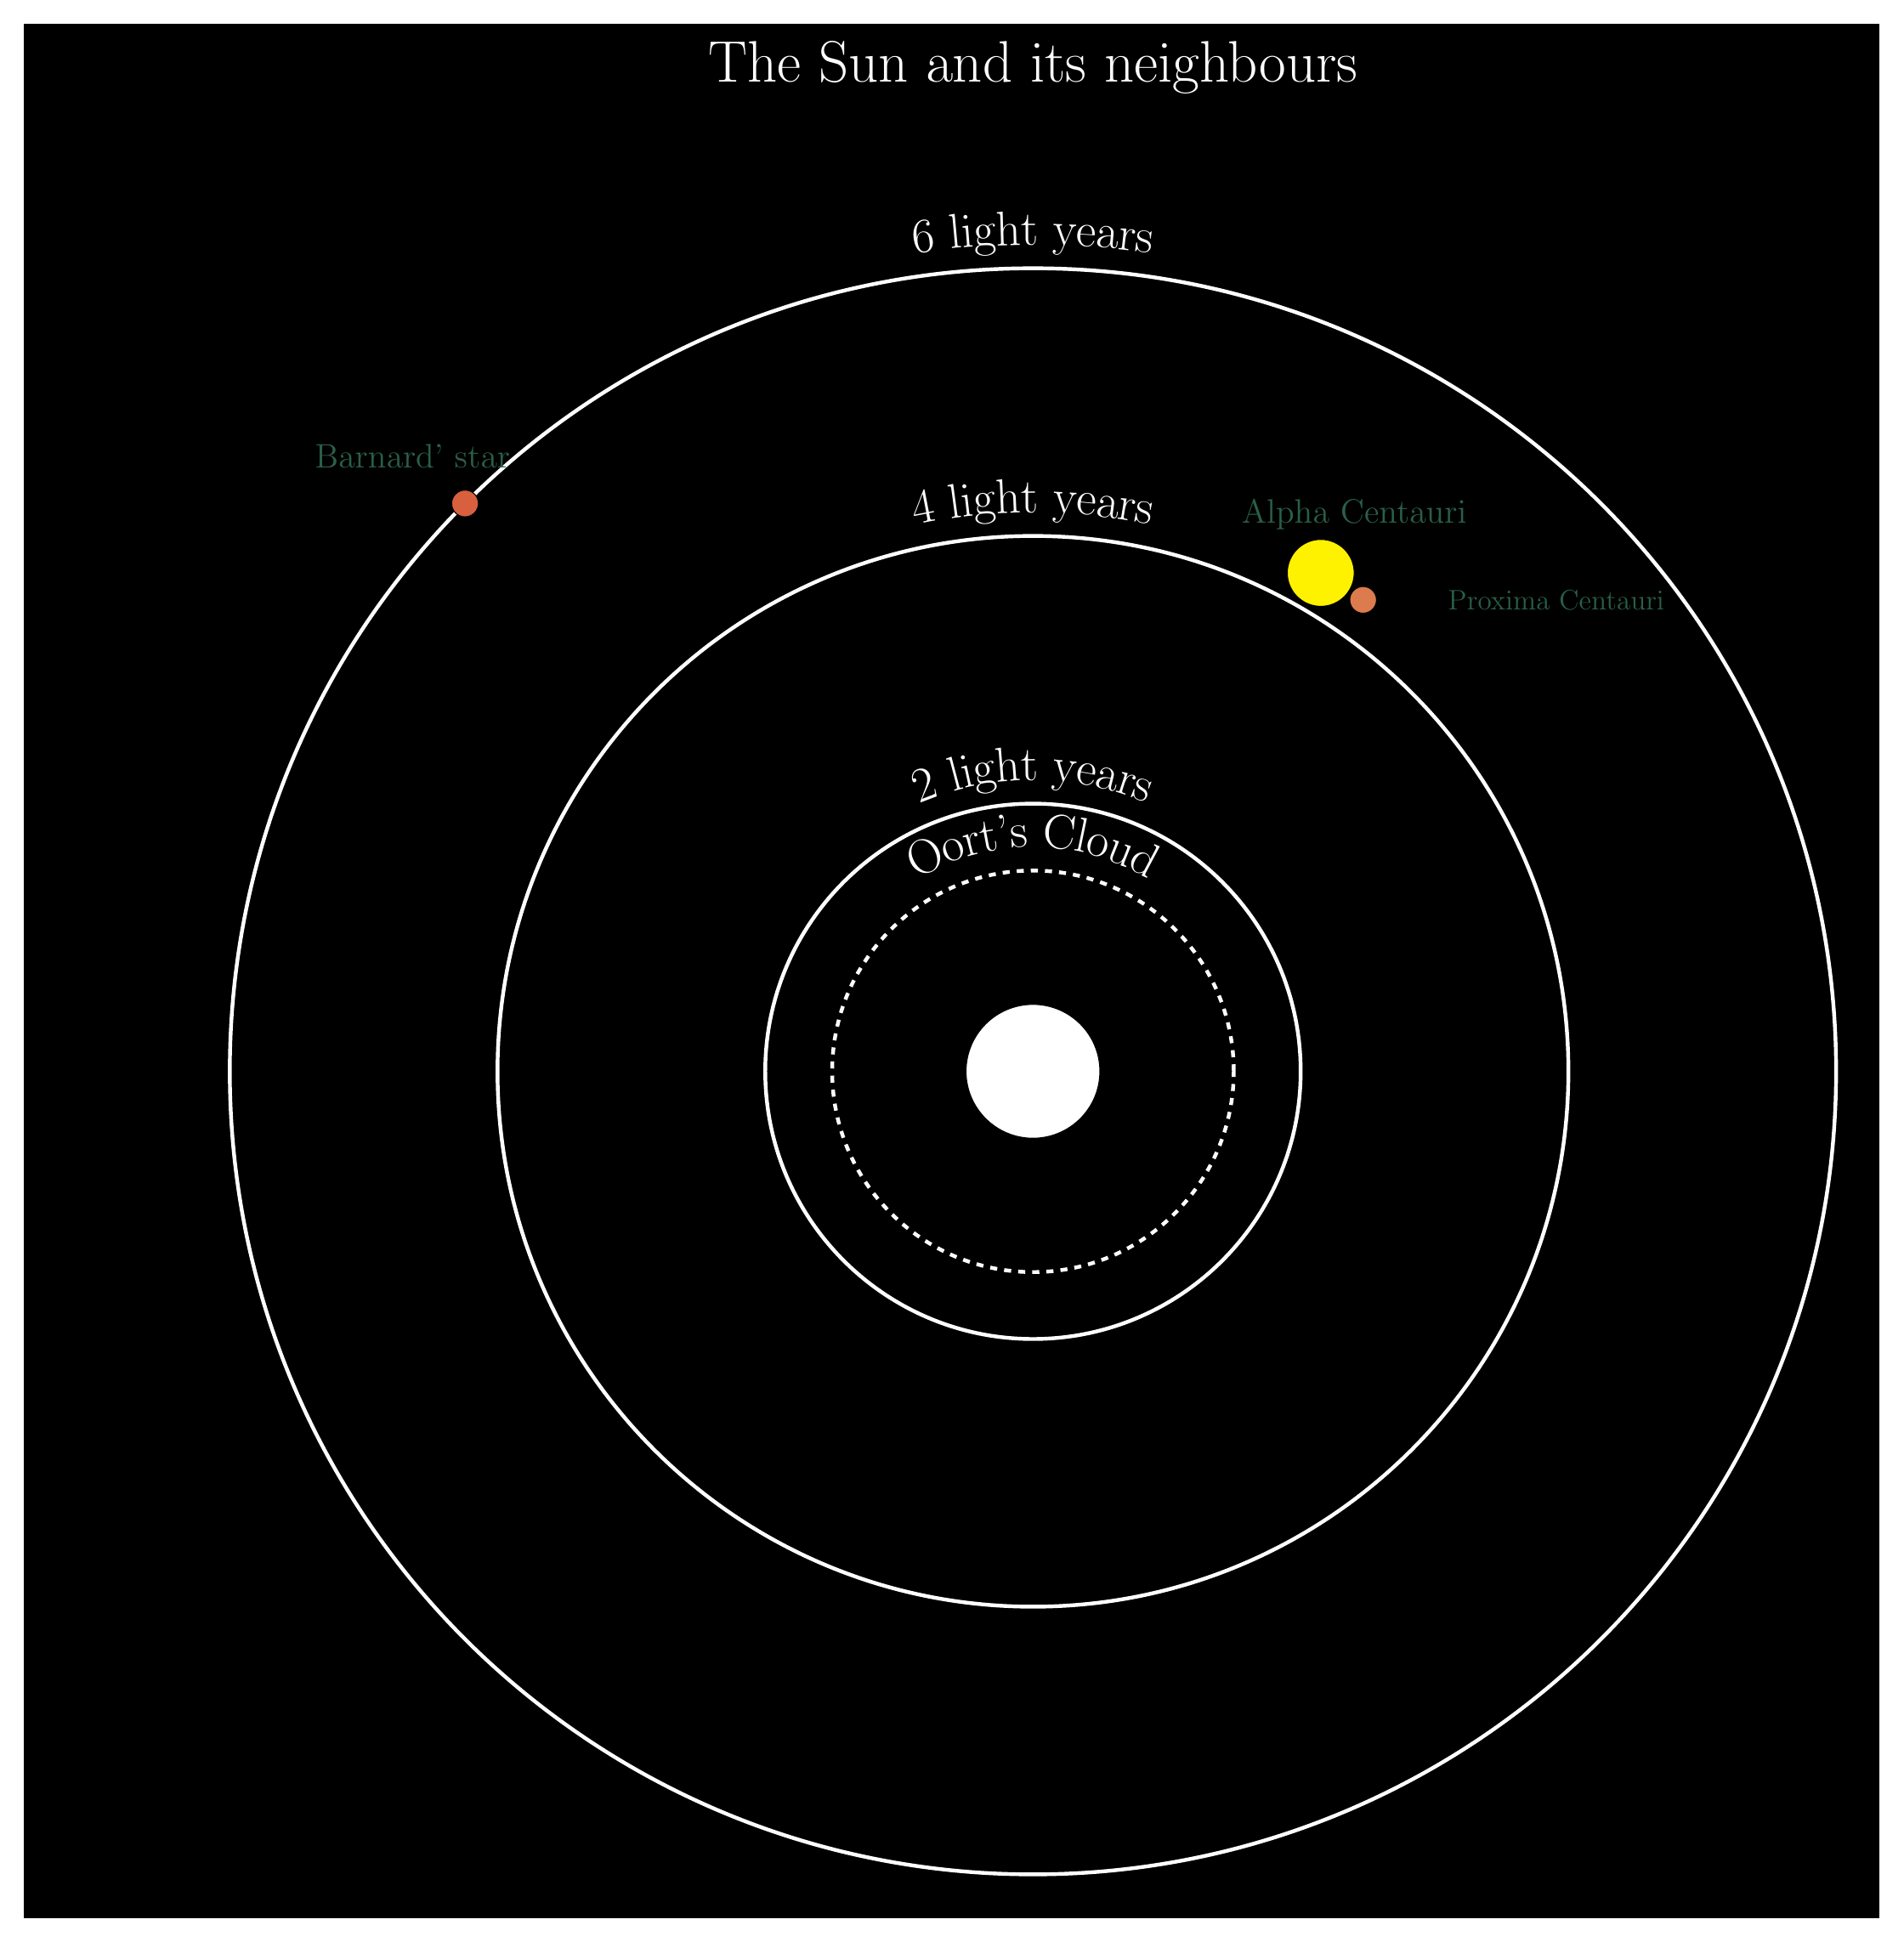
\begin{tikzpicture}[background rectangle/.style={fill=black},show background rectangle]
		\begin{scope}
			\node at (0,0) {\textcolor{white}{\fontsize{32}{33}\selectfont The Sun and its neighbours}};
		\end{scope}
		\begin{scope}[shift={(0,-15)}]
			\tkzDefPoint(0,0){S}
			\tkzDefPoint(0,12){B}
			\tkzDefPoint(-1.5,14.5){Bu}
			\tkzDefPoint(0,8.6){AC}
			\tkzDefPoint(0,9.6){ACu}
			\tkzDefPoint(0,8.6){PC}
			\tkzDefPointBy[rotation= center S angle 45](B) \tkzGetPoint{B1}
			\tkzDefPointBy[rotation= center S angle 45](Bu) \tkzGetPoint{Bu1}
			\tkzDefPointBy[rotation= center S angle -30](AC) \tkzGetPoint{AC1}
			\tkzDefPointBy[rotation= center S angle -30](ACu) \tkzGetPoint{ACu1}
			\tkzDefPointBy[rotation= center S angle -35](PC) \tkzGetPoint{PC1}
			%
			\def\myshift#1{\raisebox{-2.5ex}}
			\draw [fill=white] (S) circle (1cm);
			\draw [ultra thick, dashed, color=white] (S) circle (3cm);
			\path [postaction={decorate,decoration={raise=-1ex,text along path, reverse path,text align=center, text={|\huge\color{white}\fontsize{17}{18}|Oort's Cloud}}},rotate around={-90:(S)}] (S) circle (3.5cm);
			%
			\draw [ultra thick, color=white] (S) circle (4cm);
			\path [postaction={decorate,decoration={raise=-1ex,text along path, reverse path,text align=center, text={|\huge\color{white}\fontsize{17}{18}|2 light years}}},rotate around={-90:(S)}] (S) circle (4.5cm);
			%
			\draw [ultra thick, color=white] (S) circle (8cm);
			\path [postaction={decorate,decoration={raise=-1ex,text along path, reverse path,text align=center, text={|\huge\color{white}\fontsize{17}{18}|4 light years}}},rotate around={-90:(S)}] (S) circle (8.5cm);
			%
			\draw [ultra thick, color=white] (S) circle (12cm);
			\path [postaction={decorate,decoration={raise=-1ex,text along path, reverse path,text align=center, text={|\huge\color{white}\fontsize{17}{18}|6 light years}}},rotate around={-90:(S)}] (S) circle (12.5cm);
			%
			\draw [fill=lsb] (B1) circle (0.2cm);
			%
			\node (example-textwidth-2) [align=right, text width=7cm, color=starname, font=\fontsize{15pt}{16pt}\selectfont] at (Bu1) {Barnard' star};
			%
			\draw [fill=yellow] (AC1) circle (0.5cm);
			\draw [fill=mars] (PC1) circle (0.2cm);
			%
			\node (example-textwidth-2) [align=center, text width=7cm, color=starname, font=\fontsize{15pt}{16pt}\selectfont] at (ACu1) {Alpha Centauri};
			%
			\node (example-textwidth-2) [align=right, text width=9cm, color=starname, font=\fontsize{13pt}{14pt}\selectfont] at (PC1) {Proxima Centauri};
		\end{scope}
	\end{tikzpicture}
\end{document}